\documentclass[polish,10pt]{beamer}
\usepackage[T1]{fontenc}
\usepackage{polski}
\usepackage{babel}
\usepackage{amsmath}
\usepackage{mathtools}

\usetheme{Frankfurt}
\title{Operacje na macierzach}
\author{Valerija Artiomova 287111}

\begin{document}

\maketitle

\begin{frame}
    \frametitle{Spis treści}
    \tableofcontents[]
\end{frame}

\section{Operacje na macierzach}
\begin{frame}{Operacje na macierzach}
Podstawowe operacje na macierzach:
    \begin{enumerate}
        \item Dodawanie 
        \item Mnożenie
        \item Transpozycja
        \item Obliczanie wyznacznika
        \item Odwracanie
    \end{enumerate}
\end{frame}

\subsection{Dodawanie}
\begin{frame}{Dodawanie}
    \begin{definition}
        Suma dwóch macierzy $A \in M_{n \times m}(\mathbb{R})$ i $B \in M_{n \times m}(\mathbb{R})$ jest równa macierzy $C \in M_{n \times m}(\mathbb{R})$, której każdy element jest opisany następującym wzorem:
        \begin{equation*}
            c_{i j} = a_{i j} + b_{i j}
        \end{equation*}
    \end{definition}
    
    \begin{gather*}
        C= \begin{bmatrix}
                a_{1,1} & a_{1,2} & \cdots & a_{1,n} \\
                a_{2,1} & a_{2,2} & \cdots & a_{2,n} \\
                \vdots  & \vdots  & \ddots & \vdots  \\
                a_{m,1} & a_{m,2} & \cdots & a_{m,n} 
            \end{bmatrix}
        +
            \begin{bmatrix}
                b_{1,1} & b_{1,2} & \cdots & b_{1,n} \\
                b_{2,1} & b_{2,2} & \cdots & b_{2,n} \\
                \vdots  & \vdots  & \ddots & \vdots  \\
                b_{m,1} & b_{m,2} & \cdots & b_{m,n} 
            \end{bmatrix}\\
        =   \begin{bmatrix}
                a_{1,1} + b_{1,1} & a_{1,2} + b_{1,2} & \cdots& a_{1,n} + b_{1,n} \\
                a_{2,1} + b_{1,1} & a_{2,2} + b_{2,2} & \cdots& a_{2,n} + b_{2,n} \\
                \vdots  & \vdots  & \ddots & \vdots  \\
                a_{m,1} + b_{m,1} & a_{m,2} + b_{m,2} & \cdots& a_{m,n} + b_{m,n}
            \end{bmatrix}
    \end{gather*}
\end{frame}

\subsection{Mnożenie}
\begin{frame}{Mnożenie}
\begin{definition}
    Jeżeli $A \in M_{l \times m}(\mathbb{R})$ i $B \in M_{m \times n}(\mathbb{R})$ są macierzami, to ich iloczyn \cite{Mnozenie_macierzy}, oznaczany $AB$, jest macierzą $C \in M_{l \times n}(\mathbb{R})$
    
    \begin{equation*}
    C = AB \text{, gdzie } 
    c_{i j} = \sum_{r=1}^{m} a_{i r}b_{r j} = a_{i 1}b_{j 1} + a_{i r}b_{r i} + \dots + a_{i r}b_{r j}
    \end{equation*}
\end{definition}
\end{frame}

\begin{frame}{Mnożenie c.d.}
    \begin{flalign*}
        A =
        \begin{bmatrix}
            a_{1,1} & a_{1,2} & \cdots & a_{1,m} \\
            a_{2,1} & a_{2,2} & \cdots & a_{2,m} \\
            \vdots  & \vdots  & \ddots & \vdots  \\
            a_{l,1} & a_{l,2} & \cdots & a_{l,m} 
        \end{bmatrix},
        B =
        \begin{bmatrix}
            b_{1,1} & b_{1,2} & \cdots & b_{1,n} \\
            b_{2,1} & b_{2,2} & \cdots & b_{2,n} \\
            \vdots  & \vdots  & \ddots & \vdots  \\
            b_{m,1} & b_{m,2} & \cdots & b_{m,n} 
        \end{bmatrix} \\
        C =
        \begin{bmatrix}
            c_{1,1} & c_{1,2} & \cdots & c_{1,n} \\
            c_{2,1} & c_{2,2} & \cdots & c_{2,n} \\
            \vdots  & \vdots  & \ddots & \vdots  \\
            c_{l,1} & c_{l,2} & \cdots & c_{l,n} 
        \end{bmatrix}
        \text{, gdzie }
        c_{i j} = \sum_{r=1}^{m} a_{i r}b_{r j}
    \end{flalign*}
\end{frame}

\begin{frame}{Mnożenie c.d.}
    \centering
    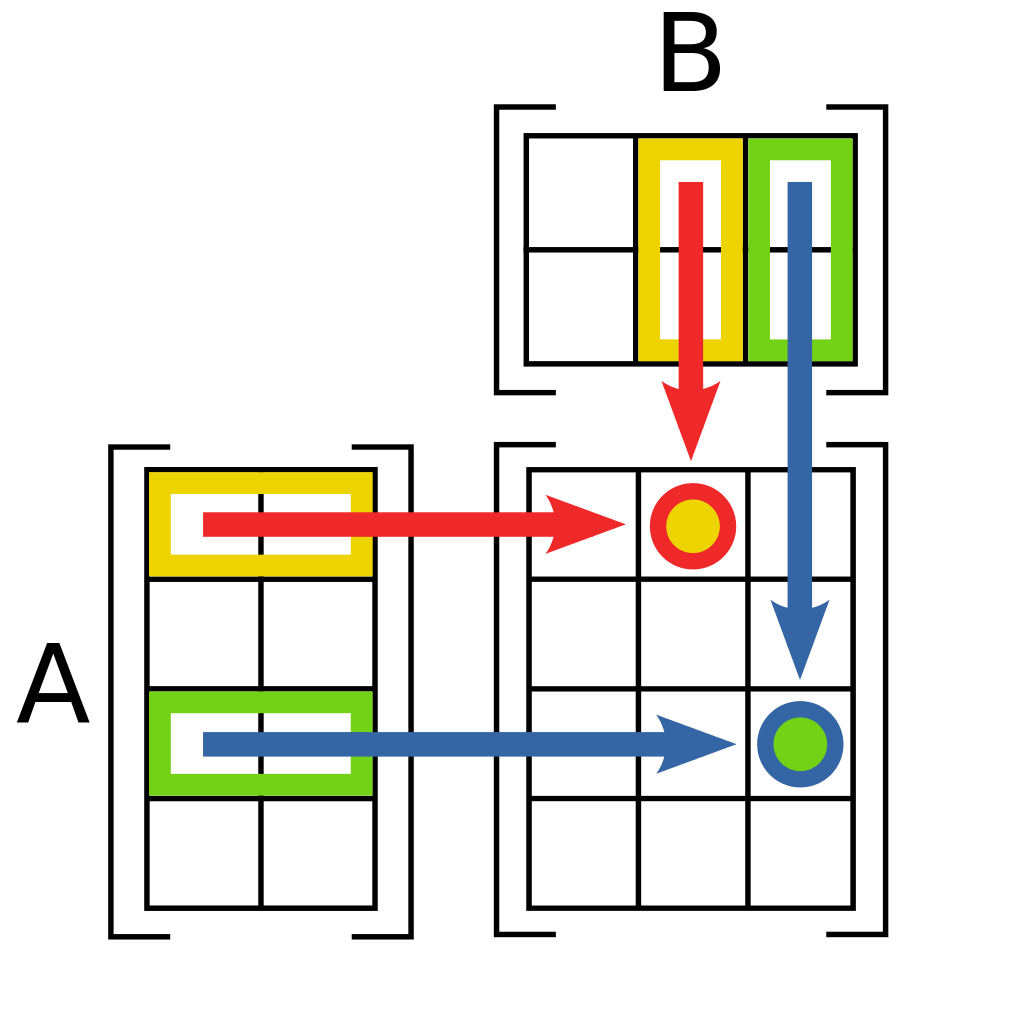
\includegraphics[width=200pt]{images/matrix_multi.png}
\end{frame}

\begin{frame}{Mnożenie - przykład}
\begin{example}
    \begin{gather*}
        \begin{bmatrix}
            3 & 6 & 1 \\
            1 & 4 & 2
        \end{bmatrix}
        \begin{bmatrix}
            1 & 5 \\
            2 & 4 \\
            1 & 3
        \end{bmatrix}
        =  \\
        \begin{bmatrix}
            3 \cdot 1 + 6 \cdot 2 + 1 \cdot 1 & 3 \cdot 5 + 6 \cdot 4 + 1 \cdot 3 \\
            1 \cdot 1 + 4 \cdot 2 + 2 \cdot 1 & 1 \cdot 5 + 4 \cdot 4 + 2 \cdot 3 \\
        \end{bmatrix}
        =
        \begin{bmatrix}
            16 & 42 \\
            11 & 27 
        \end{bmatrix}
    \end{gather*}
\end{example}
\end{frame}

\subsection{Transpozycja macierzy}
\begin{frame}{Macierz transponowana}
    \begin{definition}
        Macierz transponowana\cite{Macierz_transponowana} macierzy $A$ – macierz $A^T$ - która powstaje z danej macierzy poprzez zamianę jej wierszy na kolumny i kolumn na wiersze.
    \end{definition}
    
    \begin{example}
    \begin{equation*}
        A =
        \begin{bmatrix}
            5 & 6 & 1 \\
            8 & 0 & 2 \\
            9 & 2 & 9 \\
            3 & 4 & 7 \\
        \end{bmatrix}
        A^T = 
        \begin{bmatrix}
            5 & 8 & 9 & 3 \\
            6 & 0 & 2 & 4 \\
            1 & 2 & 9 & 7\\
        \end{bmatrix}
    \end{equation*}
    \end{example}
\end{frame}

\subsection{Wyznacznik}
\begin{frame}{Wyznacznik}
\begin{definition}
    Pierścień przemienny (komutatywny) – pierścień, w którym mnożenie jest przemienne, czyli którego wszystkie elementy ze sobą komutują, tj. dla dowolnych elementów $a$, $b$ danego pierścienia $\mathbb{R}$ zachodzi \begin{equation*}
        a \cdot b = b \cdot a
    \end{equation*}
\end{definition}
\begin{definition}
    Wyznacznikiem \cite{Wyznacznik} nazywamy funkcję przyporządkowującą każdej macierzy kwadratowej $A \in M_{n \times n}(\mathbb{R})$ o współczynnikach z pierścienia przemiennego $\mathbb{R}$ pewien element tego pierścienia.
    Wyznacznik macierzy kwadratowej $A$ oznaczany jest przez $|A|$, $\det A$, czasem tez $\Delta(A)$.
\end{definition}
\end{frame}

\begin{frame}{Wyznacznik c.d.}
    \begin{definition}[Definicja permutacyjna]
    Niech $A \in M_{n \times n}(\mathbb{R})$ jest macierzą. Wówczas:
    \begin{equation*}
        \det A = \sum_{\sigma \in S_n} (-1)^{Inv(\sigma)} a_{1 {\sigma(1)}} a_{2 {\sigma(2)}} \cdots a_{n {\sigma(2n)}}
    \end{equation*}
    gdzie $S_n$ oznacza zbiór wszystkich permutacji zbioru ${1,2,\cdots,n}$, zaś $Inv(\sigma)$ oznacza liczbę inwersji danej permutacji $\sigma \in S_n$
    \end{definition}
    
    \begin{definition}[Definicja rekurencyjna]
    Niech $A \in M_{n \times n}(\mathbb{R})$ jest macierzą.Wyznacznikiem macierzy nazywamy funkcję $\det:M_{n \times  n}(\mathbb{R})) \to \mathbb{R})$ spełniająca:
    \begin{enumerate}
        \item jeśli $n=1$, to $\det A = a_{1 1}$
        \item jeśli n >1, to $\det A = \sum_{i=1}^{n} (-1)^{i+j}a_{i j}\det A_{i j}$, gdzie $i$ jest dowolną liczbą naturalną z zakresu $1 \leq j \leq n$, a przez $A_{i j}$ oznaczamy macierze stopnia n-1, powstałą z macierzy A poprzez skreślenie $i$-tego wiersza i $j$-tej kolumny (minor).
    \end{enumerate}
    \end{definition}
\end{frame}

\begin{frame}{Wyznacznik c.d.}
\begin{example}
        \begin{equation*}
            \det \begin{bmatrix}
                a & c \\
                b & d
            \end{bmatrix} 
            = (-1)^{1+1}ad + (-1)^{1+2}cb = ad - cb
        \end{equation*}
        
        Przykładowo:
        \begin{equation*}
            \det \begin{bmatrix}
                1 & 2 \\
                4 & 3
            \end{bmatrix} 
            = 3 - 8 = -5
        \end{equation*}
    \end{example}
   \begin{center}
    \begin{tabular}{ |c|c| }
        \hline
        
\includegraphics[width=50pt]{images/det_1.png} & 
\includegraphics[width=100pt]{images/det_2.png} \\
        \hline
    \end{tabular}
    \end{center}
\end{frame}

\subsection{Odwracanie}
\begin{frame}{Odwracanie macierzy}
\begin{definition}
    Niech $A$ jest macierzą kwadratową ustalanego stopnia. Macierz $A$ jest odwracalna, jeżeli istnieje taka macierz $B$, że zachodzi:
    \begin{equation*}
        AB = BA = I
    \end{equation*}
\end{definition}

Własności
\begin{itemize}
    \item Macierz odwrotna \cite{Macierz_odwrotna} do macierzy odwracalnej jest odwracalna, operacja odwracania macierzy jest inwolucją
    \begin{equation*}
        (A^{-1})^{-1} = A
    \end{equation*}
    
    \item Iloczyn macierzy odwracalnych jest macierzą odwracalną (kolejność macierzy jest istotna)
    \begin{equation*}
        (AB)^{-1} = A^{-1}B^{-1}
    \end{equation*}
    
    \item Jeżeli macierz $A$ jest odwracalna, to także $A^{T}$ jest odwracalna
    \begin{equation*}
        (A^T)^{-1} = (A^{-1})^T
    \end{equation*}
    
\end{itemize}
\end{frame}

\begin{frame}{Odwracanie macierzy c.d.}
    \begin{example}[Metoda operacji elementarnych]
\begin{equation*}
    [A|I] \to [I|A^{-1}]
\end{equation*}
    \begin{equation*}
    A = \begin{bmatrix}
        1 & 2 \\
        3 & 4 \\
        \end{bmatrix},
            A^{-1} = \begin{bmatrix}
         -2 & 1 \\
         \frac{3}{2} & -\frac{1}{2} \\
        \end{bmatrix}
    \end{equation*}   
    
    \begin{gather*}
    A|I = \begin{bmatrix}
        1 & 2 & \bigm| & 1 & 0 \\
        3 & 4 & \bigm| & 0 & 1 \\
        \end{bmatrix}
        \to
        \begin{bmatrix}
        1 & 2  & \bigm| &1  & 0 \\
        0 & -2 & \bigm| & -3 & 1 \\
        \end{bmatrix}
        \to \\
        \begin{bmatrix}
        1 & 2 &\bigm| & 1 & 0 \\
        0 & 2 &\bigm| & 3 & -1 \\
        \end{bmatrix}
        \to
        \begin{bmatrix}
        1 & 0 &\bigm| & -2 & 1 \\
        0 & 2 &\bigm| & 3 & -1 \\
        \end{bmatrix}
        \to
        \begin{bmatrix}
        1 & 0 &\bigm| &-2 & 1 \\
        0 & 1 &\bigm| &\frac{3}{2} & -\frac{1}{2} \\
        \end{bmatrix}
    \end{gather*}
    \end{example}
\end{frame}

\section{Bibliografia}
\begin{thebibliography}{4}

\bibitem{Mnozenie_macierzy}
Mnożenie macierzy, online: \url{https://pl.wikipedia.org/wiki/Mno%C5%BCenie_macierzy}, dostęp: 03.02.2022

\bibitem{Wyznacznik}
Wyznacznik, online: \url{https://pl.wikipedia.org/wiki/Wyznacznik}, dostęp: 03.02.2022

\bibitem{Macierz_odwrotna}
Macierz odwrotna, online: \url{https://pl.wikipedia.org/wiki/Macierz_odwrotna}, dostęp: 03.02.2022

\bibitem{Macierz_transponowana}
   Macierz transponowana, online: \url{https://pl.wikipedia.org/wiki/Macierz_transponowana}, dostęp: 03.02.2022

\end{thebibliography}
\end{document}
